\chapter{Material}

\section{Das \rv{} zum Pendeln}

\subsection{Wieso ein \rv{} zum Pendeln?}

Es gibt durchaus Gründe, wieso man ein Trekking- oder Fitness-Bike als
ideales Pendler-Rad sehen kann \cite{Lindthaler2015perfektesfahrradpendler}.
Dieser Meinung kann ich mich nicht anschliessen. Dies aus mehreren Gründen:

\begin{itemize}
  \item Mit keiner anderen Art Fahrrad ist das Vorwärtskommen so schnell und energiesparend.
  \item Um möglichst ein funktionelles Training zu erreichen, soll dieses möglichst mit dem
    gleichen Gerät erfolgen, wie das Training selbst.
  \item Mit wenig Aufwand lässt sich ein \rv{} in ein vollwertiges Pendler-Rad umrüsten.
    Der Aufwand ist meines Erachtens kleiner, als ein Fitness-Bike zu <<versportlichen>>.
  \item Fahren mit dem \rv{} ist einfach geil, es gibt nichts anderes!
\end{itemize}

\subsection{Das ideale \rv{} zum Pendeln}

Was ist das ideale \rv{} für einen täglichen, harten Pendlereinsatz?
Die beste Grundlage dazu liefert meines Erachtens ein solides und
günstiges \rv{}. Es soll also nicht zu teuer sein (Diebstahl), darf
durchaus unscheinbar sein (selber Grund). Gerade Alu-Rahmen sind
aktuell ziemlich <<out>>, und deshalb günstig zu haben. In den
einschlägigen Online-Plattformen\footnote{\url{http://www.ricardo.ch},
\url{http://www.ebay.ch}} oder lokalen Velobörsen gibt es dazu reichlich
Auswahl. Für ein paar hundert Euro bekommt man so ein neuwertiges oder wenig
gebrauchtes \rv{}, dass der Vorbesitzer wegen Nicht-Gebrauchs abzugeben bereit
ist (siehe Abb. \ref{fig:optimales-pendler-rennvelo}).

Neben der richtigen Grösse sollte man noch auf Standart-Komponenten achten
(Shimano), um den Unterhalt möglichst günstig zu halten.

Da ein Pendler-\rv{} allwettertauglich sein muss, gehört ein Spritzschutz
daran. Es gibt dazu sehr leichte, schmale Kunststoff-Teile. In der Regel
werden diese mit Gummi-Zügen festgemacht, da empfielt sich eine stabilere
Befestigung mit Kabelbindern.

Was auch wichtig ist, sind \emph{zwei} Bidon-Halter. Einer für das
tatsächliche Bidon und einen für einen Reparatur-Bidon.

Sichtbarkeit wird verbessert mit Leucht-Klebern. Auch hier lohnt sich der
Einsatz eines speziellen Pendler-Rades -- die Hemmung, das schöne Bike mit
Leucht-Klebern zuzupflastern wird dadurch kleiner.

Clipless- oder normale Pedalen? Ist wohl auch eine Glaubensfrage. Für ein
Pendler-\rv{} das vor allem in der Stadt gefahren wird, finde ich persönlich
normale Pedalen praktischer. Clipless-Pedalen wären am \rv{} natürlich ein
Muss, sind aber wg. dem dazu nötigen Schuhwerk etwas umständlicher.

Licht am \rv{} ist natürlich unverzichtbar. Am besten eignet sich dazu
natürlich entsprechende Zubehörteile mit Akku. Dieses Thema wird in einem
eigenen Abschnitt behandelt.

\begin{figure}[htpb]
        \centering
        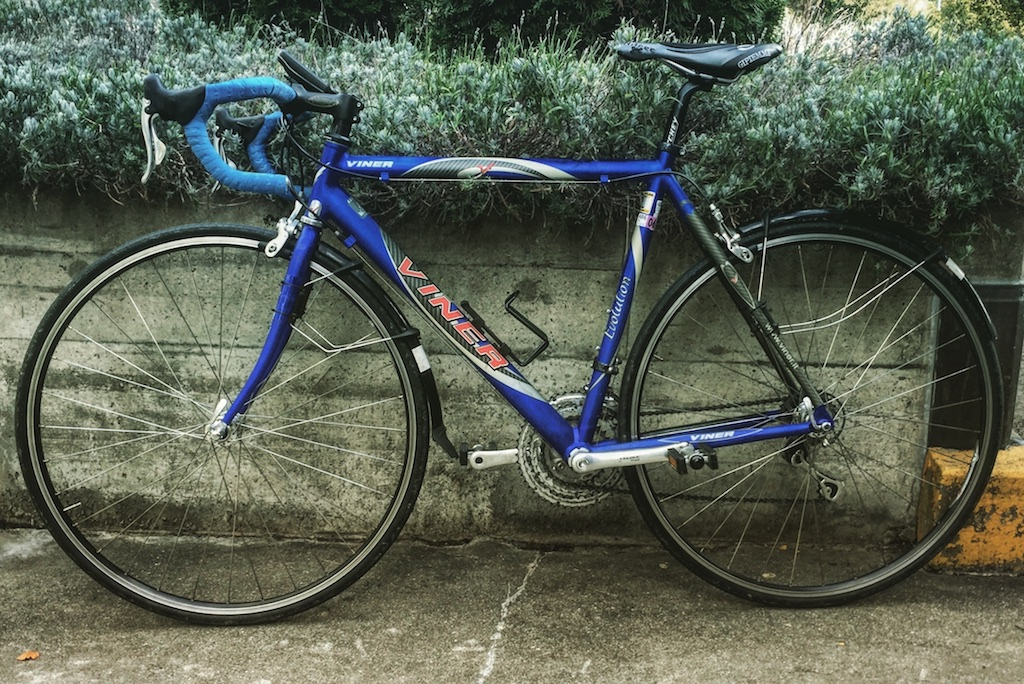
\includegraphics[width=\textwidth]{figures/optimales-pendler-rennvelo.jpg}
        \caption{Ein günstiges, gebrauchtes \rv{} mit Spritzschutz und normalen Pedalen
            als ideales Pendler-Instrument. Ein, besser zwei, Bidon-Halter sind praktisch.}
        \label{fig:optimales-pendler-rennvelo}
\end{figure}

\section{Regelmässige Wartung des \rv}

Das \rv{} muss regelmässig gewartet werden. Das dient der Pannensicherheit und der Langlebigkeit.

Je länger man mit Wartungsarbeiten zuwartet, desto umfagreicher werden
erfahrungsgemäss die Reparaturen. Auch eine wichtige Erfahrung: wenn einem
beim Fahren etwas auffällt (Geräusch, komisches Gefühl), dann sollte man
unbedingt dem nachgehen. Ignorieren oder Verdrängen (<<Da wird schon nichts
sein>>) bringt \emph{todsicher} Probleme. Irgendwann ist dann die lockere
Schraube ganz weg und eine Reparatur, die bei besserer Aufmerksamkeit ein paar
Sekunden gedauert hätte, wird ein Steckenbleiben am blödsten Ort und eine
umfangreiche und teure Reparatur.

In absteigender Reihenfolge sollen Reparatur- und Unterhaltsarbeiten am \rv{} folgendermassen 
erledigt werden:

\begin{enumerate}
  \item Vor Ort:
    Das Mitführen von Reparaturzeugs für Platten usw. ist obligatorisch.
    Alles was abschliessend repariert werden kann, sind <<Notlösungen>> (z.B. Reparaturspray) vorzuziehen.
    Schlechte Erfahrungen habe ich ach gemacht, mit so. <<Selbstreparierenden>> Schlauchlösungen.
    Die halten den Druck für einen Rennradreifen nicht aus, sind schwer und teuer und nutzlos.
    Lieber gleich dauerhaft Reparieren, das spart auf die Länge an Zeit.
    Die Reparatur eines Plattens ist mit etwas Übung (und einem Ersatzschlauches) in 10-15 Minuten
    erledigt. Auch hier ist eine gute, mentale Grundeinstellung hilfreich.
    Pannen passieren. Anstatt sich zu ärgern sich ein bequemes, gutes Plätzchen suchen und sich
    ruhig und systematisch an die Analyse des Problems und dessen Behebung widmen.
    Siehe Abb. \ref{fig:reparatur-unterwegs}.
  \item Am Arbeitsplatz:
    Gelegentlich passiert einem etwas auf dem Weg zur Arbeit. Wenn man das \rv
    dann reparieren kann, erspart man sich viel umtriebe (Transport des nicht
    mehr fahrtauglcihen Rades nach Hause, dortige Reparatur).
    Glücklich ist, wer am Arbeitsplatz ein kleines Reparaturset hat -- ev. das ausgesonderte
    Doppel von zu Hause. So können wichtige Reparaturen gleich über Mittag erledigt werden.
    Siehe Abb. \ref{fig:reparatur-arbeitsplatz}.
  \item Zu Hause nach der Arbeit:
    Es braucht Überwindung, am Abend noch Zeit in die Wartung zu investieren, man sollte es
    aber der Sicherheit wegen schon tun.
    Dazu gehört natürlich auch der Ersatz von gebrauchtem Reparaturmaterial und die Reparatur
    von defekten und austetauschten Schläuchen.
  \item Am Wochenende:
    Das Wochenende soll den grösseren Reparatur- und Unterhaltsarbeiten vorbehalten bleiben.
    So z.B. Tausch der Kette, Wartung der Lager usw.
\end{enumerate}

\begin{figure}[htpb]
        \centering
        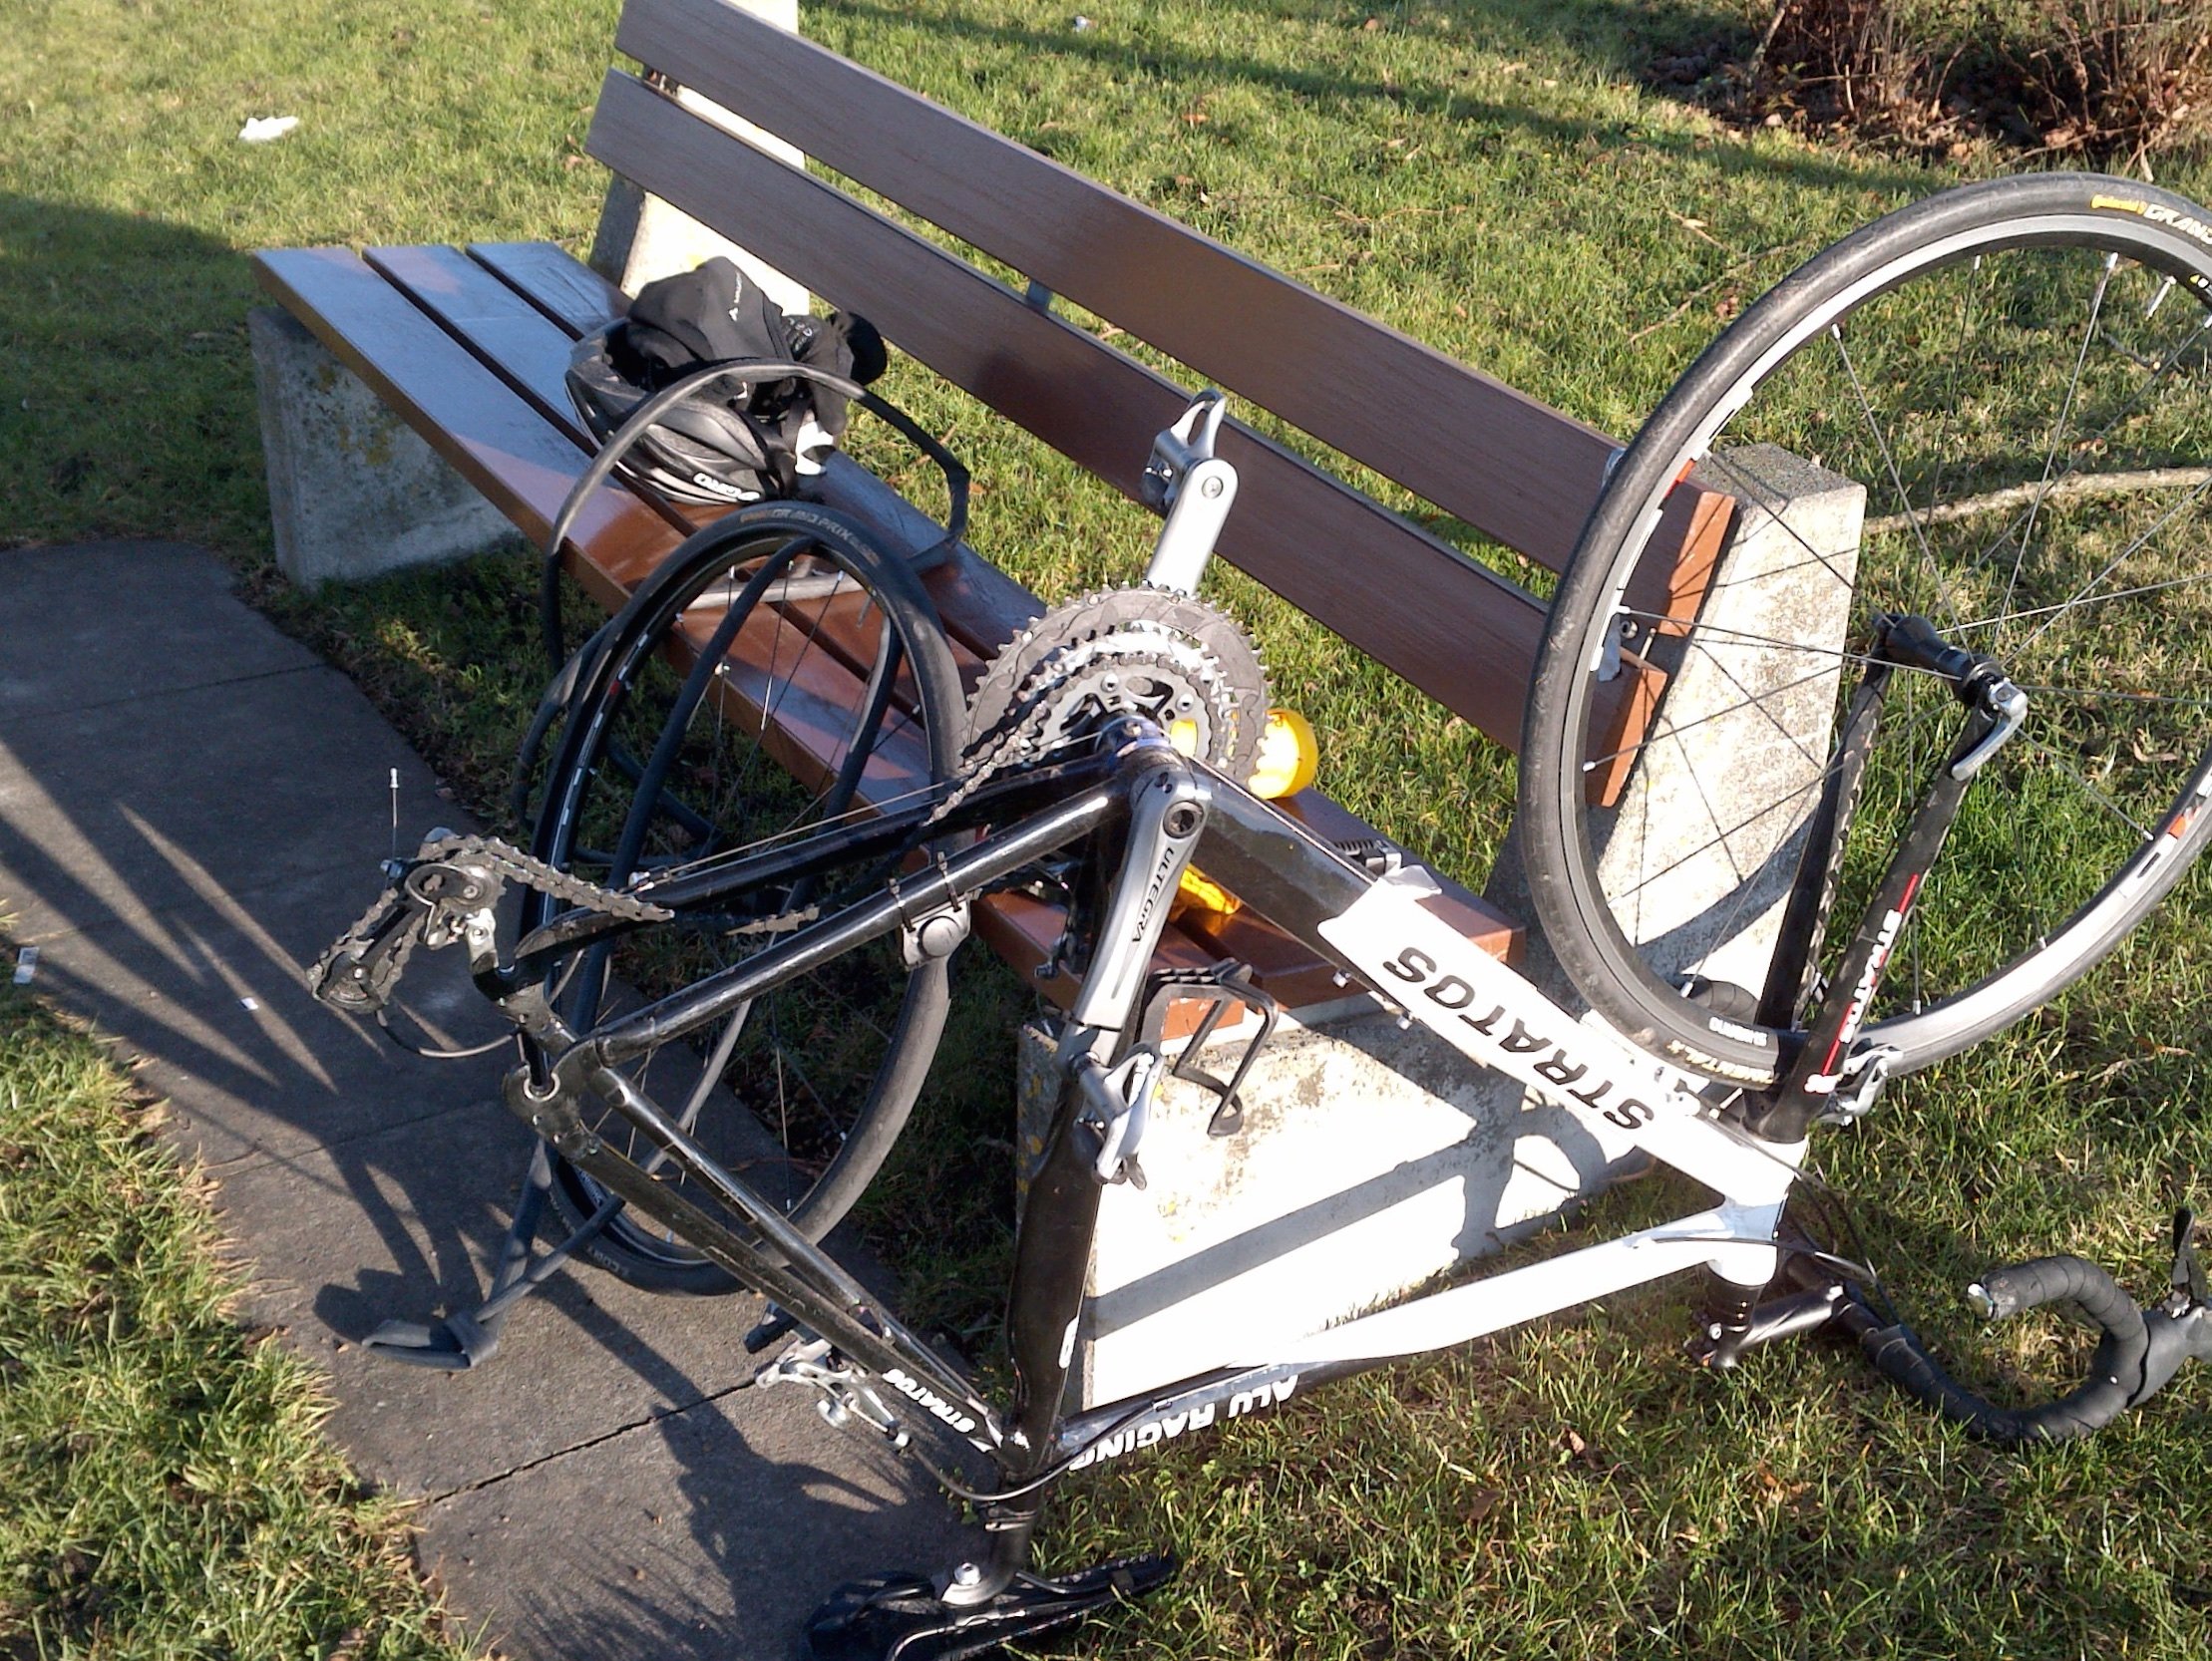
\includegraphics[width=0.8\textwidth]{figures/reparatur-unterwegs.jpg}
        \caption{Reparatur unterwegs}
        \label{fig:reparatur-unterwegs}
\end{figure}

\begin{figure}[htpb]
        \centering
        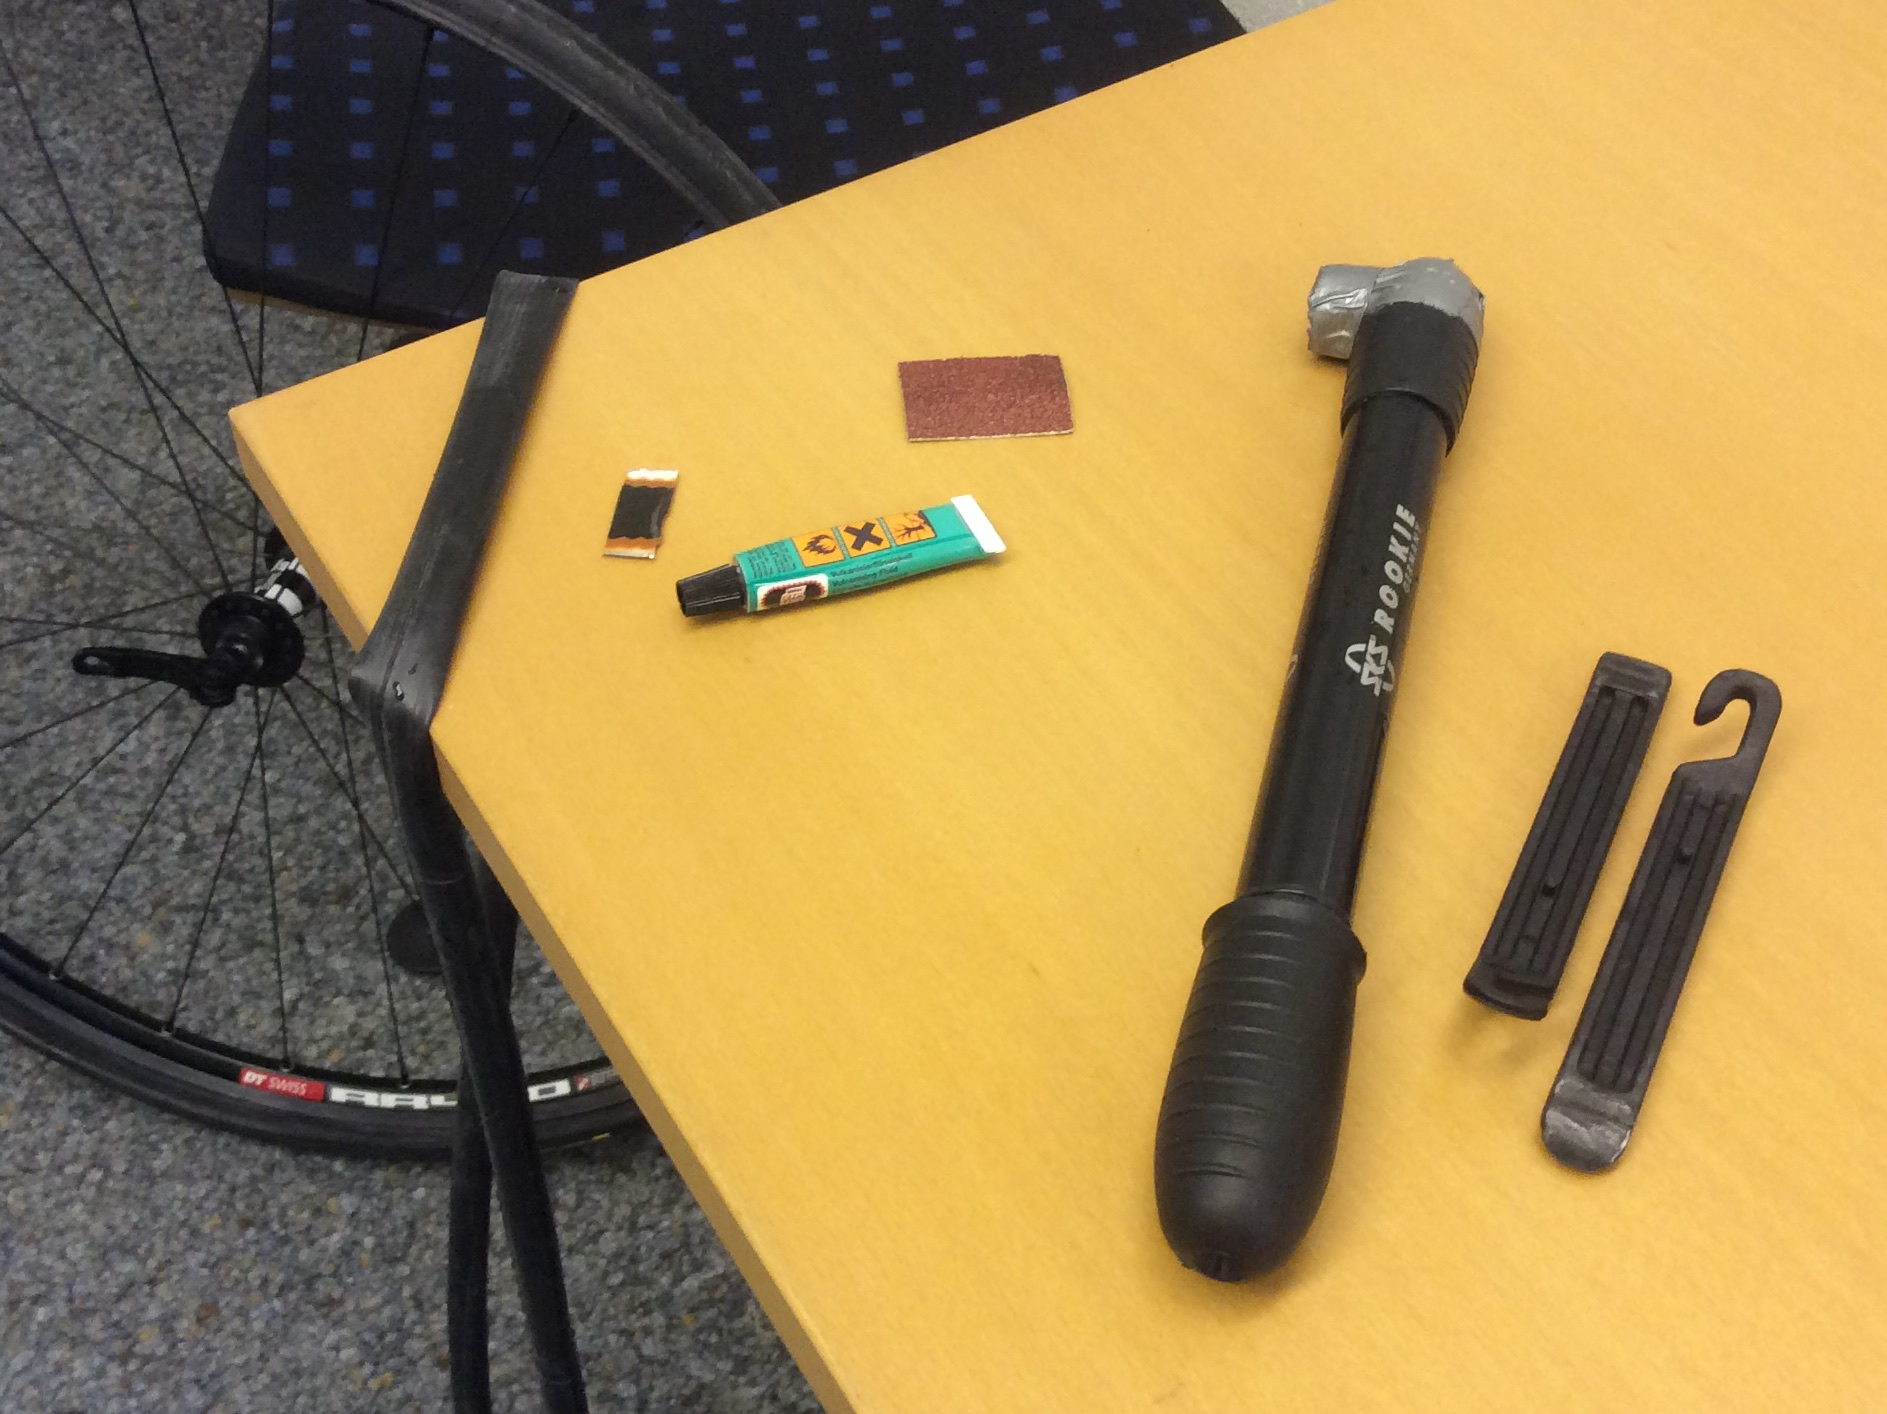
\includegraphics[width=0.8\textwidth]{figures/reparatur-arbeitsplatz.jpg}
        \caption{Reparatur am Arbeitsplatz}
        \label{fig:reparatur-arbeitsplatz}
\end{figure}

\section{Bekleidung}

Der Fokus ist hier eher bei einer multifunktonalen Outdoor-Bekleidung
als einer \emph{stilsicheren} Rennradbekleidung.
So kann man durchaus auch bei MTB-Klamotten oder Outdoor-Sachen fündig werden.

Schuhe mit weicher Sohle sind hartsohligen Rennradschuhen vorzuziehen.

Überschuhe als Regenschutz.
